\section{Linear Latent Variable Models}

  Note that in PCA, we have taken some data $x$ in high-dimension $D$ and reduced it to a lower-dimensional orthogonal representation in $\mathbb{R}^k$. In other words, the corresponding $z$ represents $x$ in another space, which we call a \textbf{latent space}. This concept of representing data from one space to another are called \textbf{factor analysis}, or \textbf{latent variable analysis}, and is an extremely important concept for state-of-the-art models. 

  Say that we want to do density estimation for the probability distribution of the covariates $X$, a random variable. We can try to model it directly, but this may be infeasible. Rather, what we do is ``add" a latent distribution $Z$, creating the joint distribution $(X, Z)$. This may look more complicated, but make two simplifying assumptions: we hope that we can model the latent $Z$ in a simple form (like a Gaussian), and we can model the conditional probability $p(x \mid z)$ as some function $f_\theta$ parameterized by $\theta$. We can therefore marginalize and find that 
  \begin{equation} 
    p_X (x) = \int_{z \in \mathbb{R}^k} p (x \mid z) \, p_Z (z) \,dz = \mathbb{E}_Z [p(X \mid Z)] 
  \end{equation}

  Like we do with everything else in math, we take a look at the simplest example: linear functions. In \textbf{linear factor models}, we start with the unknown covariate distribution $X \in \mathbb{R}^d$, and we create a latent variable $Z \in \mathbb{R}^k$ with some simple assumed distribution $Z \sim p_Z (z)$.\footnote{Usually, we also constrain it to be factorable (i.e. is the product of its marginal distributions: $p(z) = \prod_i p(z_i)$) so that it is easy to sample from. Occasionally, the stronger assumption of the $z_i$'s being iid is made.} For general latent variable models, we have a \textbf{latent transform} $g: \mathbb{R}^k \rightarrow \mathbb{R}^d$ that links the two distributions together as $X = g(Z)$. Then, we assume that 
  \begin{equation}
    X = \mu + W Z + \epsilon
  \end{equation}
  where the noise $\epsilon$ is typically Gaussian and diagonal (but not necessarily the same component-wise variances). Finally, we can use techniques like MLE to estimate $W, \mu$, and the parameters of $\epsilon$. 

  The entire reason we want to do this is that we are hoping that we can construct a complex distribution $X$ from a simple distribution $Z$ with $d >> k$, connected by some well-studied function $X = g(Z)$. In the linear case, $W \in \mathbb{R}^{d \times k}$, and the latent variables $z$ give a more compact, parsimonious  explanation of dependencies between the components of the observations $x$. 

  \begin{definition}[Factor Analysis] 
    Factor analysis is a specific case of a linear factor model where 
    \begin{equation}
      X = \mu + WZ + \epsilon, \text{ where } z \in \mathcal{N}(0, I), \epsilon \sim \mathcal{N} \big(0, \mathrm{diag}(\sigma_1^2, \ldots, \sigma_k^2) \big)
    \end{equation}
    It should be clear to us that $X$ should be Gaussian\footnote{Since linear transformations of Gaussians are Gaussian} and that $\mathbb{E}[X] = \mu$, with 
    \begin{align} 
        \mathrm{Var}[X] & = \mathbb{E}[ (X - \mu)(X - \mu)^T ] \\
                        & = \mathbb{E}[ (W Z + \epsilon) (Z^T W^T + \epsilon^T)] \\
                        & = \mathbb{E}[W z z^T W^T] + \mathbb{E}[ \epsilon \epsilon^T] \\
                        & = W \mathbb{E}[ z z^T] W^T + \mathbb{E}[ \epsilon \epsilon^T] \\
                        & = W W^T + \mathrm{diag}(\sigma_1^2, \ldots, \sigma_d^2) 
    \end{align} 
    The $W, \mu$, and $\sigma_i$'s can be estimated using MLE methods. Unfortunately, no closed form  exists, so iterative methods are commonly applied. 
  \end{definition} 

\subsection{Probabilistic PCA}

  We want to take PCA and extend it to be a \textit{generative model}, which allows you to sample data. In regular PCA, we saw that for some $z \in \mathbb{R}^k$ in the latent space, $\hat{x} = \mu + V_k \Sigma_k z$. Therefore, if we just change $z$ from a point to a probability distribution (e.g. Gaussian), we can take a random variable $z \sim \mathcal{N}(0, I)$ from $\mathbb{R}^k$, and then transform it to get a random variable $x = \mu + V^T \sigma_k z$, which will give a density. 
  \begin{equation}
    x \sim \mathcal{N} \big( \mu, V^T \Sigma_k (V^T \Sigma_k)^T \big) = \mathcal{N} \big( \mu, X_k^T X_k)
  \end{equation} 
  Note that in here, $X$ is a random variable that we are trying to fit to the data $X_k$. However, $X_k \in \mathbb{R}^{k \times n}$ with $k << n$, and so $X_k^T X_k \in \mathbb{R}^{n \times n}$ is not full rank, and so the distribution is restricted to strictly the $k$-dimensional subspace $L_k \subset \mathbb{R}^D$. We want to add a bit of noise beyond the subspace, so we add an extra small Gaussian $\epsilon$ around it. In general factor analysis above, we set $\epsilon$ to have an arbitrary diagonal Gaussian, but we just use an isotropic one $\epsilon \sim \mathcal{N}(0, \sigma^2 I )$, giving us 
  \begin{equation}
    X = \mu + V_k \Sigma_k Z + \epsilon \implies X \sim \mathcal{N} \big( \mu, X_k X_k^T + \sigma^2 I)
  \end{equation} 
  Note that PPCA is really a specific instance of factor analysis, and we assume that the latent variable $z$ follows a standard Gaussian $\mathcal{N}(0, 1)$. It turns out that this extension has the flaw that the subspace generated by the MLE estimate of $X$ will not necessarily correspond to the principal subspace of the data. But we can make this happen with one more assumption. 

  \begin{definition}[Probabilistic PCA] 
    The \textbf{probabilistic PCA} model is a latent factor model of form  
    \begin{equation}
      x \sim \mathcal{N}(\mu, W W^T + \sigma^2 I) 
    \end{equation} 
    with the latent transform 
    \begin{equation}
      X = g_{\mu, W, \sigma} (Z) = \mu + (WW^T + \sigma^2 I )^{1/2} Z
    \end{equation}
  \end{definition} 

  Optimizing this model is actually quite easy. 

  \begin{theorem}[MLE of PPCA Model]
    Given $X^{(i)} \sim X$ iid, the MLEs for $W, \mu, \sigma$ are 
    \begin{align}
      \mu_{MLE} & = \frac{1}{N} \sum_{i=1}^N X^{(i)} \implies \hat{\mu}_{MLE} = \frac{1}{N} \sum_{i=1}^N x^{(i)} \\ 
      \hat{\sigma}^2_{MLE} & = \frac{1}{d-k} \sum_{j=k+1}^d \lambda_j \\
      W_{MLE} & = U_q (\Lambda_d - \hat{\sigma}_{MLE}^2 I_d )^{1/2} R
    \end{align}
  \end{theorem}
  \begin{proof}
    Given $X^{(i)} \sim X$ iid, the MLEs for $W, \mu, \sigma$ have a closed form, and model parameter estimation can be performed iteratively and efficiently. We have 
    \begin{equation}
      \mu_{MLE} = \frac{1}{N} \sum_{i=1}^N X^{(i)} \implies \hat{\mu}_{MLE} = \frac{1}{N} \sum_{i=1}^N x^{(i)}
    \end{equation}
    and setting the biased MLE estimator of the variance, 
    \begin{equation}
      \widehat{\mathrm{Var}}_{MLE}(\mu_{MLE}) = S = \frac{1}{N} \sum_{i=1}^N (X^{(i)} - \mu_{MLE}) (X^{(i)} - \mu_{MLE})^T
    \end{equation}
    we can derive the MLE of $W$.\footnote{Note that $W_{MLE}$ is not unique. Say that $W^\ast$ is an MLE, then, for any unitary $U \in \mathbb{R}^{k \times k}$, we have $W^\ast W^{\ast T} = (W^\ast U) (W^\ast U)^T$.} We can find the MLE estimate of $\sigma$ first by taking a look at $C = \mathrm{Var}[X] = W W^T + \sigma^2 I$. It is the sum of positive semidefinite patrices that are also symmetric, so by the spectral theorem it is diagonalizable and has full rank $d$. But $W W^T$ is rank $k$, so $d - k$ of the eigenvalues of $W W^T$ is $0$, indicating that the same $d-k$ smallest eigenvalues of $C$ is $\sigma^2$. Therefore, we can take the smallest $d-k$ eigenvalues of our MLE estimator of $C$, which is $S$, and average them to get our MLE for $\sigma$. 
    \begin{equation}
      \hat{\sigma}^2_{MLE} = \frac{1}{d-k} \sum_{j=k+1}^d \lambda_j
    \end{equation}
    We can approximate $W W^T = C - \sigma^2 I \approx S - \hat{\sigma}^2_{MLE} I$, and by further taking the eigendecomposition $C = U \Sigma U^T \implies W W^T = U (\Sigma - \sigma^2 I) U^T$ and cutting off the last $d-k$ smallest eigenvalues and their corresponding eigenvectors, we can get 
    \begin{equation}
      W_{MLE} = U_q (\Lambda_d - \hat{\sigma}_{MLE}^2 I_d )^{1/2} R
    \end{equation}
    where the $R$ just accounts for any unitary matrix. 
  \end{proof}

  Now as $\sigma \rightarrow 0$, the density model defined by PPCA becomes very sharp around these $d$ dimensions spanned by the columns of $W$. At $0$, our MLE of $W$ is simplified and we have 
  \begin{equation}
    X = W_{MLE} z + \mu_{MLE} + \epsilon = U_q \Lambda_q^{1/2} z + \mu_{MLE}
  \end{equation}
  which essentially reduces to regular PCA. That is, the conditional expected value of $z$ given $X$ becomes an orthogonal projection of $X - \mu$ onto the subspace spanned by the columns of $W$. Intuitively, we can see that we are estimating the Gaussian, which corresponds to the mean squared distance from each $x^{(i)}$ to $\ell_k$. 

\subsection{Linear Independent Component Analysis} 

  ICA is a method to separate a multivariate signal into additive, statistically independent components. It does come with a lot of assumptions, and is a specific instance of a linear factor model where $\mu = 0$ and $\epsilon = 0$. 

  \begin{definition}[Linear ICA]
    In \textbf{linear ICA}, we have the simple model. 
    \begin{equation}
      x = W z
    \end{equation}
    In here, $X \in \mathbb{R}^d$ is a mixture vector and $W \in \mathbb{R}^{d \times k}$ is a \textbf{mixing matrix}. Both $W$ and $z$ are unknown, and we need to recover them given $x$. We have 2 strong assumptions. 
    \begin{enumerate} 
      \item Each component of $z$ is independent (not just uncorrelated). This is an easy enough assumption to intuit.  
      \item Independent components of $z$ must \textit{not} be Gaussian.\footnote{This is needed for us to be able to ``unmix'' the signals. To see why, just suppose $z$ was Gaussian, and so the vector $Rz$ is also Gaussian for any invertible $R$. Therefore, we could find an infinite number of solutions of form $x = W R^{-1} R z$ and have no way to separate them.}
    \end{enumerate}
  \end{definition}

  \begin{algo}[Fitting]
    Now let's see how linear ICA actually estimates $W$ and $z$. Once $W$ is estimated, the latent components of a given test mixture vector, $x^\ast$ is computed by $z^\ast = W^{-1} x^\ast$. So now all there's left to do is to estimate $W$, which we want to estimate so that $W^{-1} x$ is far from Gaussian. The reason for this is that given a bunch of independent non-Gaussian $h_i$'s, if we mix them with a matrix that is not $\pm I$ , then by CLT, a linear combination of random variables will tend to be Gaussian, and so for an arbitrary $W$ we would expect $x$ to be Gaussian. Therefore, what we want to do is guess some matrix $A$, and compute 
    \begin{equation}
      A x = A W h
    \end{equation}
    and if we get things right, $A \approx W^{-1}$, and the result of $A x$ would look pretty non-Gaussian. If it it not the case, then $A W$ will still be some mixing matrix, and so $A x$ would look Gaussian. So now the question reduces to how do we choose this $A$? There are multiple ways to measure non-Gaussianity: 
    \begin{enumerate} 
      \item The absolute or squared kurtosis, which is $0$ for Gaussians. This is a differentiable function w.r.t. $W$, so we can try maximizing it. This is done for the sample kurtosis, of course.  
      \item Another measure is by maximizing the neg-entropy. 
    \end{enumerate}
  \end{algo}

  There are further ambiguities with ICA regarding uniqueness of a best representation. For one, we can only estimate the latent components up to a scaling factor since we will still get
  \begin{equation}
    x = (\alpha W) (\frac{1}{\alpha} z) \text{ for some } \alpha > 0
  \end{equation}
  We can fix this by forcing $\mathbb{E}[z_i^2] = 1$. However, there is still an ambiguity for the sign of hidden components, but this is insignificant in most applications. Second, we can estimating the components up to permutation. We have 
  \begin{equation}
    x = W P^{-1} P z
  \end{equation}
  for some permutation matrix $P$. 

  \begin{figure}[H]
    \centering 
    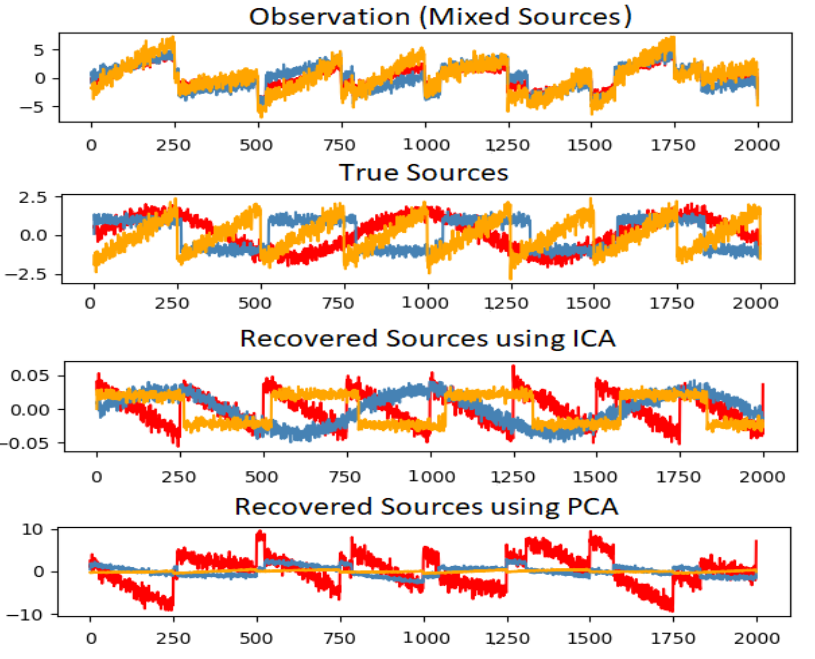
\includegraphics[scale=0.4]{img/ICA_example.png}
    \caption{We can perform this on three mixed signals with additive noise, and ICA does very well, though again some recovered signals are scaled or permuted weirdly. }
    \label{fig:}
  \end{figure}

\subsection{Slow Feature Analysis}

  Slow feature analysis also another special case of a linear factor model that uses information from time signals to learn invariant features. It is motivated by a general principle called the \textbf{slowness principle}. The idea is that the important characteristics of scenes change very slowly compared to the individual measurements that make up a description of a scene. For example, in computer vision, individual pixels can change very rapidly. If a zebra moves from left to right across the image, an individual pixel wil rapidly change from black to white. By comparison, the feature indicating whether a zebra is in the image will not change at all, and the feature describing the zebra's position will change slowly. Therefore, we want to regularize our model to learn features that change slowly over time.  

  We can apply the slowness principle to any differentiable model trained with gradient descent. That is, we can add the following term to the loss function: 
  \begin{equation}
    \lambda \sum_i d\big( f(x^{(t+1)}), f(x^{(t)}) \big)
  \end{equation}
  where $\lambda$ is a hyperparameter determining the strength of the slowness regularization term, $t$ is the time index, $f$ is the feature extractor to be regularized, and $d$ is the distance between $f(x^{(t)})$ and $f(x^{(t+1)})$. A common choice for $d$ is the mean squared difference. 

  Essentially, given a set of time-varying input signals $x^{(t)}$, SFA learns a nonlinear function $f$ that transforms $x$ into slowly-varying output signals $y$. Obviously, we can't just take some trivial function like $f = 0$, so we have the following constraints 
  \begin{align}
    \mathbb{E}_t [ f(x^{(t)})_i]  & = 0 \\ 
    \mathbb{E}_t [ f(x^{(t)})_i^2] & = 1 
  \end{align}
  \begin{center} 
    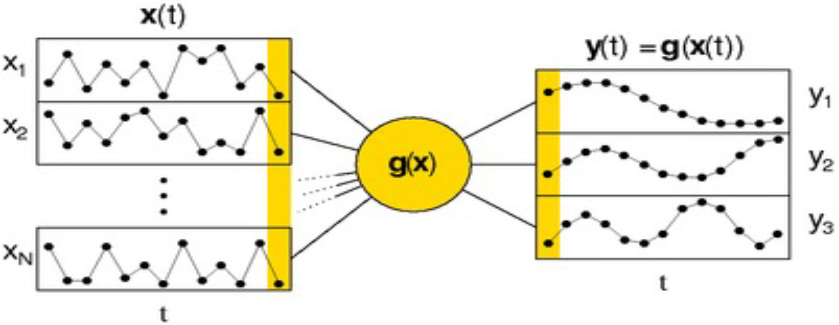
\includegraphics[scale=0.4]{img/slow_feature.png}
  \end{center}
  We can restrict the nonlinear $f$ to some subspace of functions, and this becomes a standard optimization problem where we solve 
  \begin{equation}
    \min_\theta \mathbb{E}_t \big[ \big( f(x^{(t+1)})_i - f(x^{(t)})_i \big)^2 \big]
  \end{equation}


\subsection{Latent Dirichlet Allocation} 

\subsection{Sparse Dictionary Learning} 

  Latent variables can help us represent data in lower dimensions, but another advantage is that we can get \textit{sparse} representations as well. What we want to do in sparse coding is that for each input $x^{(i)}$, we want to find a latent representation $z^{(i)}$ such that it is sparse (i.e. has many $0$s) and also we can reconstruct the original input $x^{(i)}$ well. We have basically two things to optimize: the latent representations $z$ and the decoding mechanism, which we can do with a \textit{dictionary matrix} $D$. Note that we are optimizing for \textit{both} the latent encodings and the decoding mechanism, and so this isn't a generative model. 

  \begin{definition}[Sparse Dictionary Encoding Model]
    The \textbf{sparse dictionary encoding model} is a representation model defined 
    \begin{equation}
      X = g_{D}(Z) = D Z
    \end{equation}
    where $D \in \mathbb{R}^{d \times k}$ is a \textbf{dictionary matrix} that decodes the latent $Z \in \mathbb{R}^k$ to $X \in \mathbb{R}^d$. Note that both the $z^{(i)}$'s and $D$ are optimized, so we want to perform the \textit{joint} optimization\footnote{To break this term down, let's just assume that we have a fixed dictionary $D$. Then, we just need to minimize with respect to each $h^{(t)}$. Now we can add the dictionary parameter back again. }

    \begin{equation}
      \min_{D} \frac{1}{N} \sum_{i=1}^N \min_{z^{(i)}} \underbrace{\frac{1}{2} ||x^{(i)} - D z^{(i)}||_2^2}_{\text{reconstruction error}} + \underbrace{\lambda ||z^{(i)}||_1}_{\text{sparsity penalty}}
    \end{equation}
  \end{definition}

  Note that the reconstruction, or decoding, of $x = Dz$ is linear and explicit, but if we want to encode $x \mapsto z$, we need to substitute the $x$ into the term above and minimize it w.r.t. $D$ and $z$ to solve it. Therefore, this encoder is an implicit and \textit{nonlinear} function of $x$. 

  \begin{figure}[H]
    \centering 
    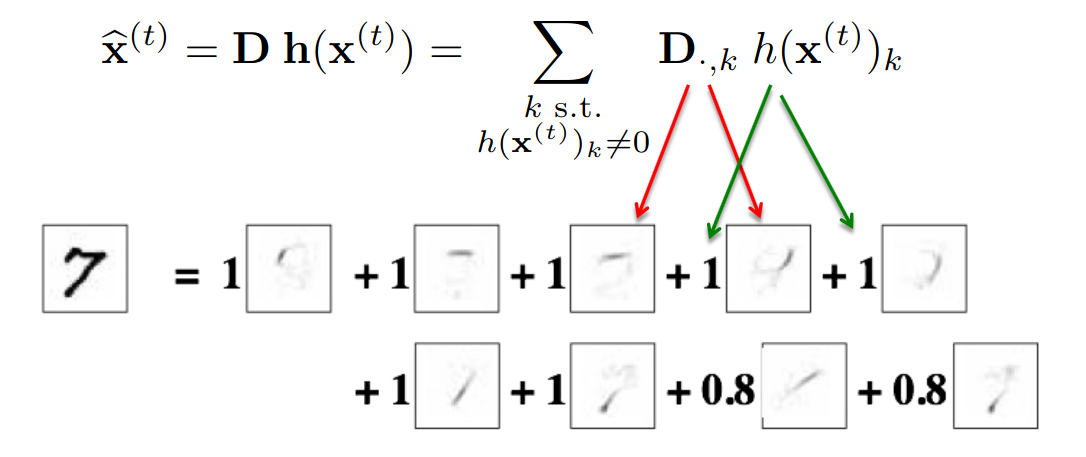
\includegraphics[scale=0.4]{img/sparse_coding.png}
    \caption{We can reconstruct an image of a seven as a linear combination of a set of images. Note that each of the images of strokes are columns of $W$ and the coefficients make up the sparse vector $h$. } 
    \label{fig:sparse_coding}
  \end{figure}

  Let's think about how we can optimize the objective function w.r.t. $h$, keeping $D$ constant. We can do stochastic gradient descent, which gives us the steps
  \begin{equation}
    \nabla_{h^{(t)}} \mathcal{L}(x^{(t)}) = D^T (D h^{(t)} - x^{(t)}) + \lambda \, \mathrm{sign}(h^{(t)})
  \end{equation}
  but this wouldn't achieve sparsity since it overshoots the $0$ all the time. Therefore, we can clip it, or we can use proximal gradient descent/ISTA to take a step, and shrink the parameters according to the L1 norm. 
  \begin{align} 
    h^{(t)} & = h^{(t)} - \alpha D^T (D h^{(t)} - x^{(t)}) \\
    h^{(t)} & = \mathrm{shrink}(h^{(t)}, \alpha \lambda)
  \end{align}
  where $\mathrm{shrink}(a, b) = [\ldots, \mathrm{sign}(a_i)\, \max(|a_i| - b_i, 0), \ldots]$. This is guaranteed to converge if $1/\alpha$ is bigger than the largest eigenvalue of $D^T D$.  

